\documentclass[12pt,letter]{article}
\usepackage{../downey_format}




\begin{document}
	
%	\large{}
%	
%	\title{\vspace{-2cm} Chapter 5: Basic concepts of Control Theory}
%	\date{}
%	\maketitle

	% set the section number, along with figure and equation numbers
	\setcounter{section}{7}	
	\setcounter{figure}{\thesection}   
	\renewcommand\thefigure{\thesection.\arabic{figure}}
	\setcounter{equation}{\thesection}   
	\renewcommand\theequation{\thesection.\arabic{equation}}

\section{Frequency Analysis}

\subsection{Time Response Under Harmonic Excitations}
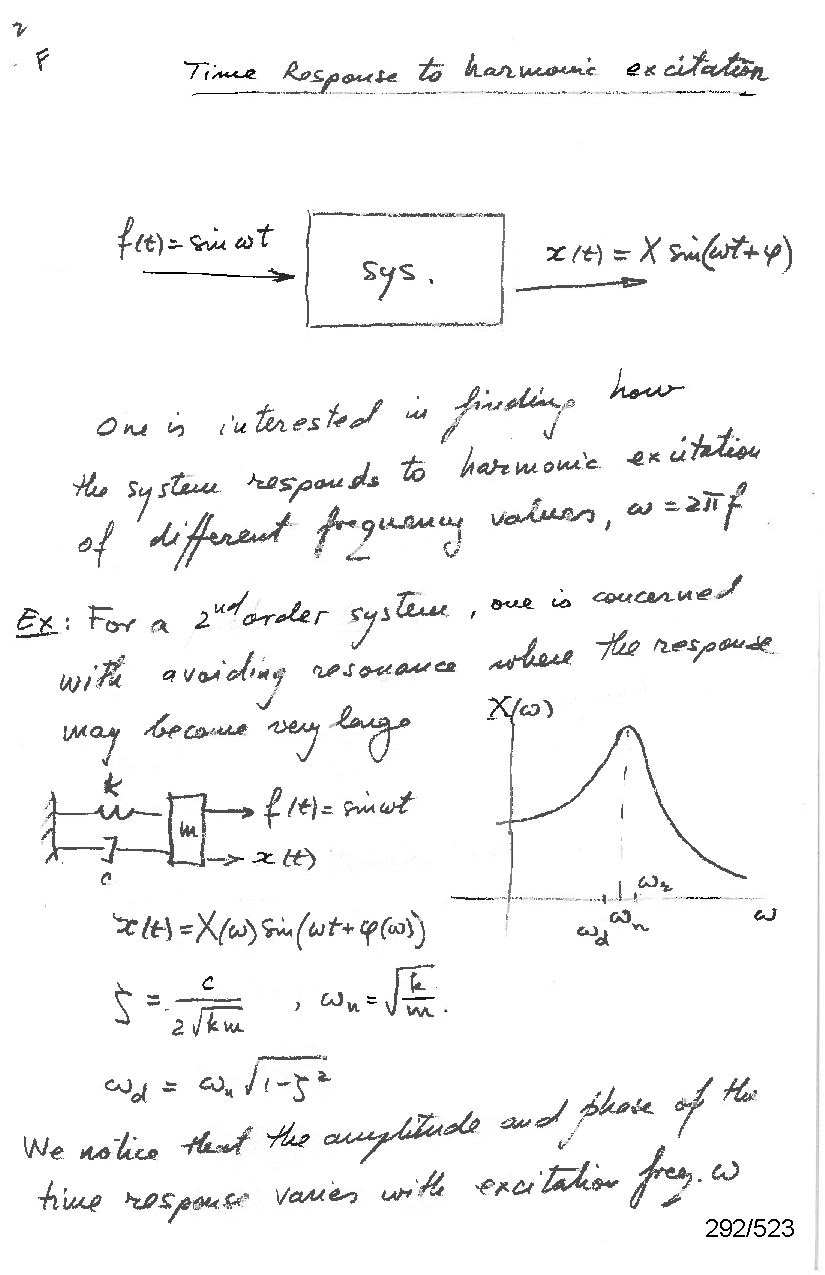
\includepdf[pages=-,pagecommand={},width=0.9\textwidth]{PDF_notes/Time_Response_Under_Harmonic_Excitations.pdf}


\subsection{Frequency Response Function (FRF)}
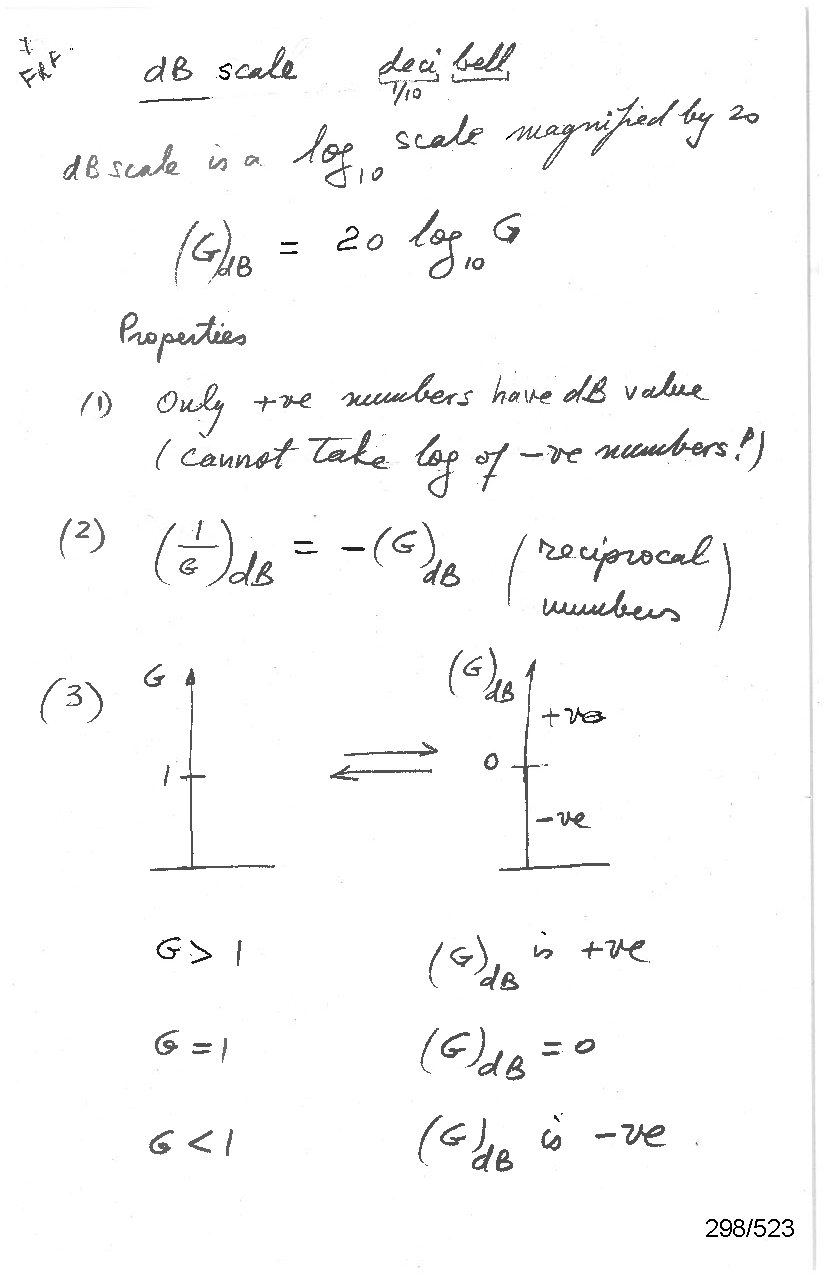
\includepdf[pages=-,pagecommand={},width=0.9\textwidth]{PDF_notes/Frequency_Response_Function.pdf}


\subsection{Performance Indicators in Frequency Domains}
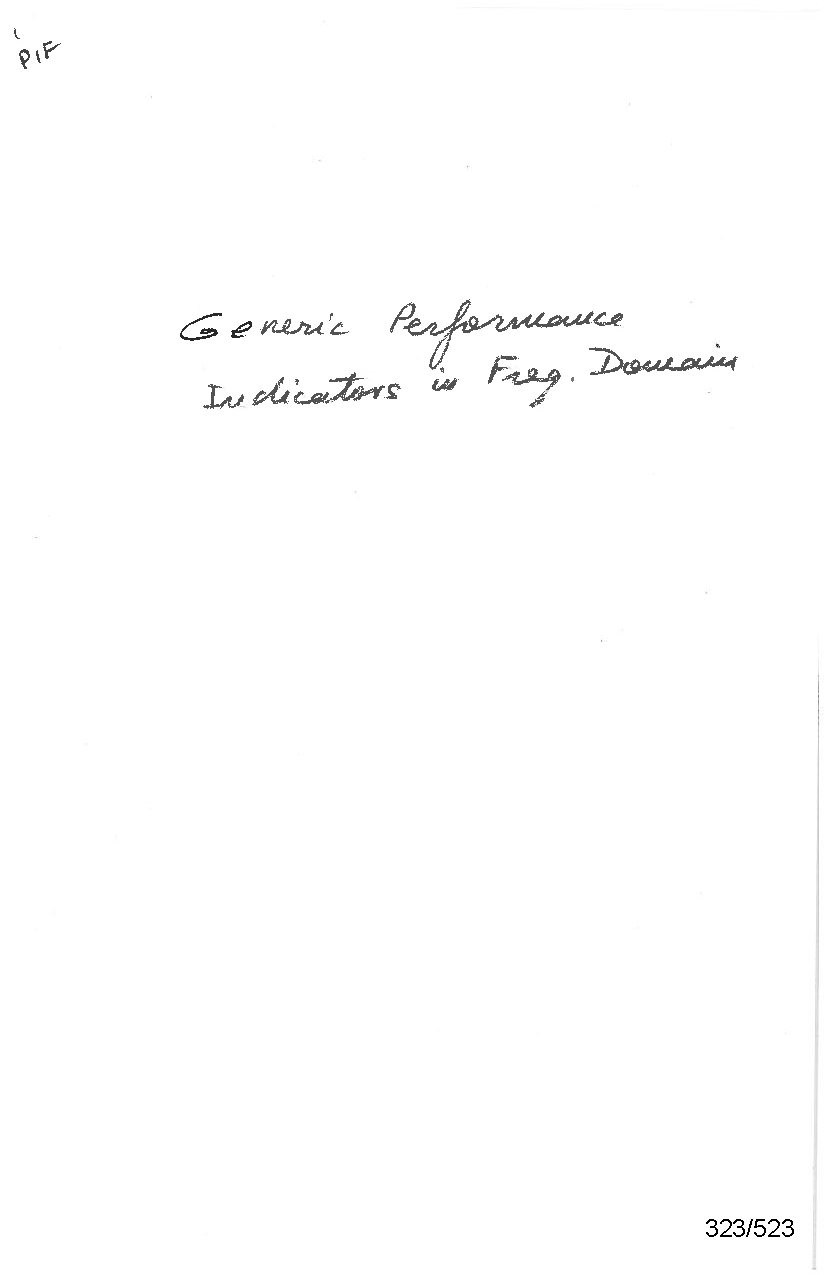
\includepdf[pages=-,pagecommand={},width=0.9\textwidth]{PDF_notes/Performance_Indicators_in_Frequency_Domains.pdf}

\subsection{System Identification in Frequency Domains}
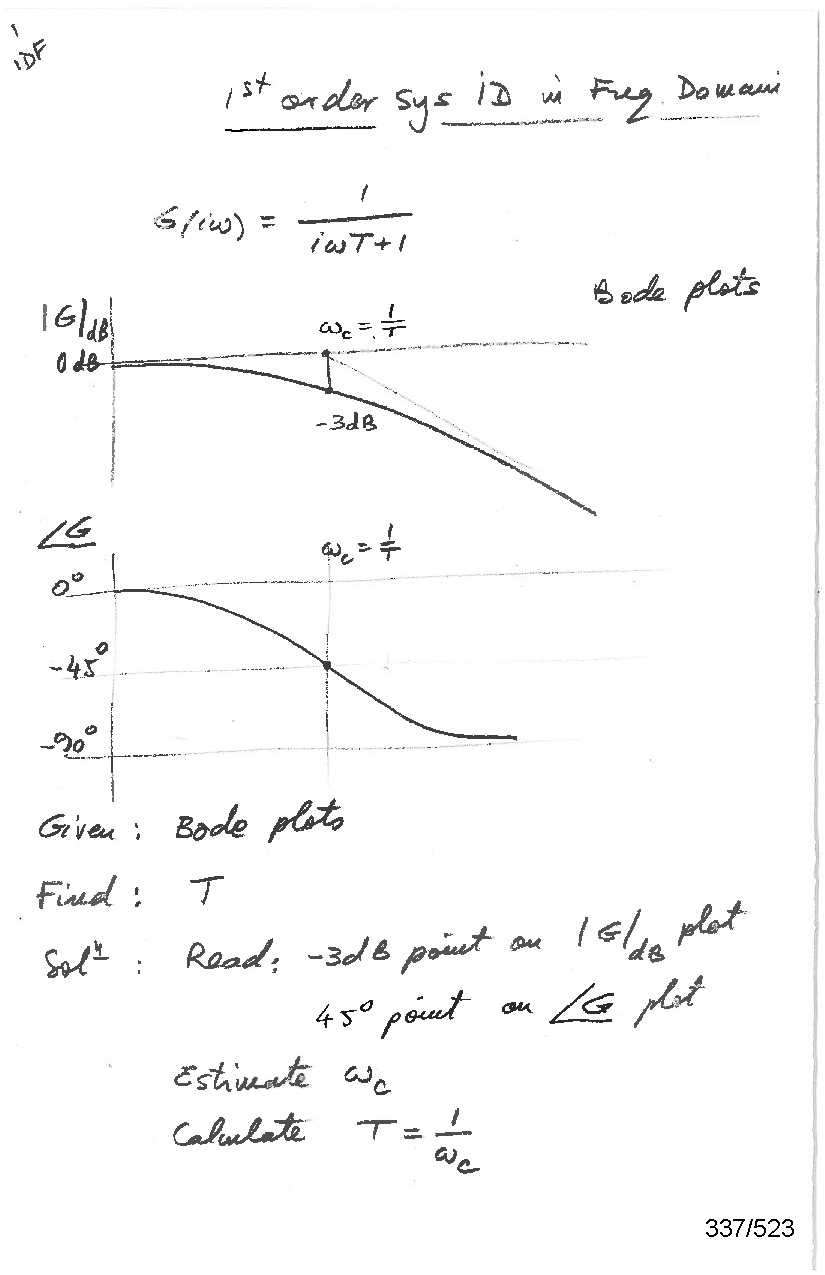
\includepdf[pages=-,pagecommand={},width=0.9\textwidth]{PDF_notes/System_Identification_in_Frequency_Domains.pdf}

\subsection{Frequency Domain Analysis of Feedback System Stability}
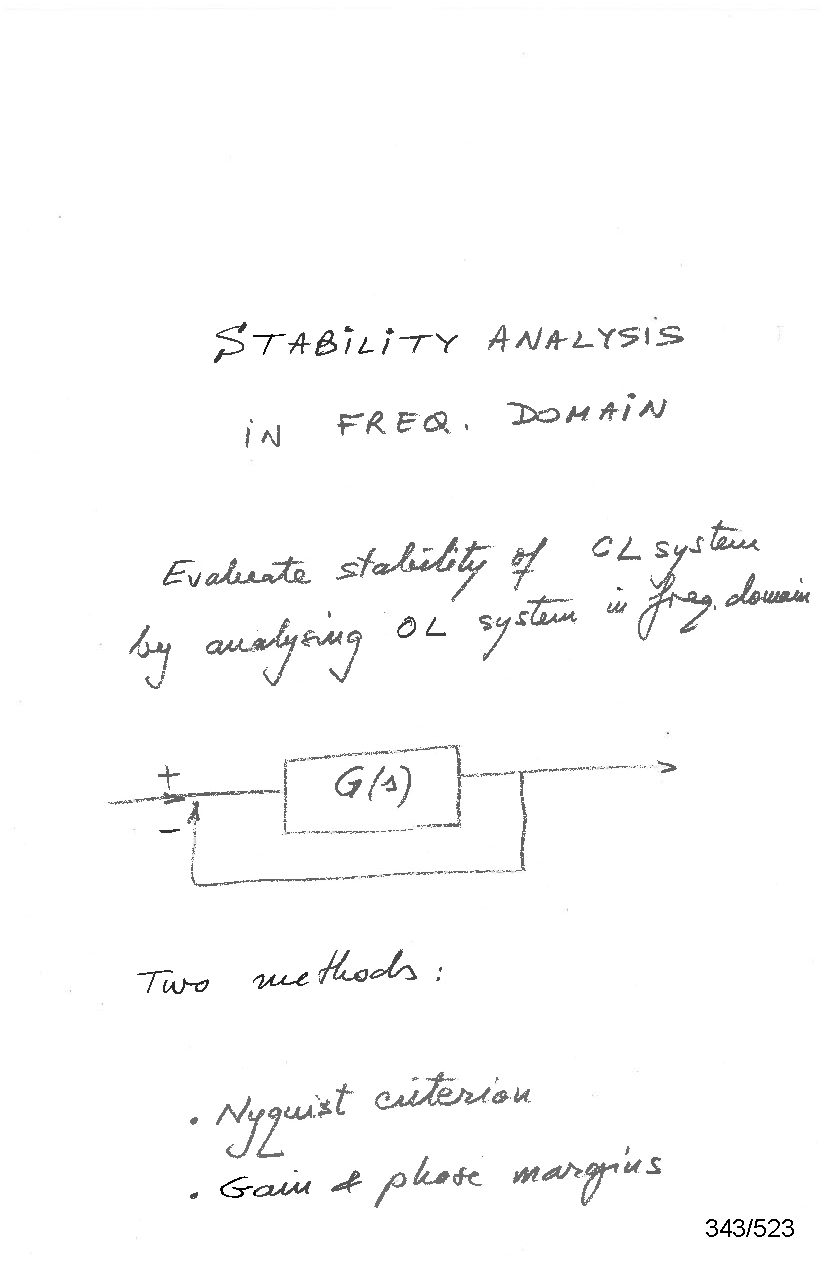
\includepdf[pages=-,pagecommand={},width=0.9\textwidth]{PDF_notes/Frequency_Domain_Analysis_of_Feedback_System_Stability.pdf}

\subsection{Stability Margins}
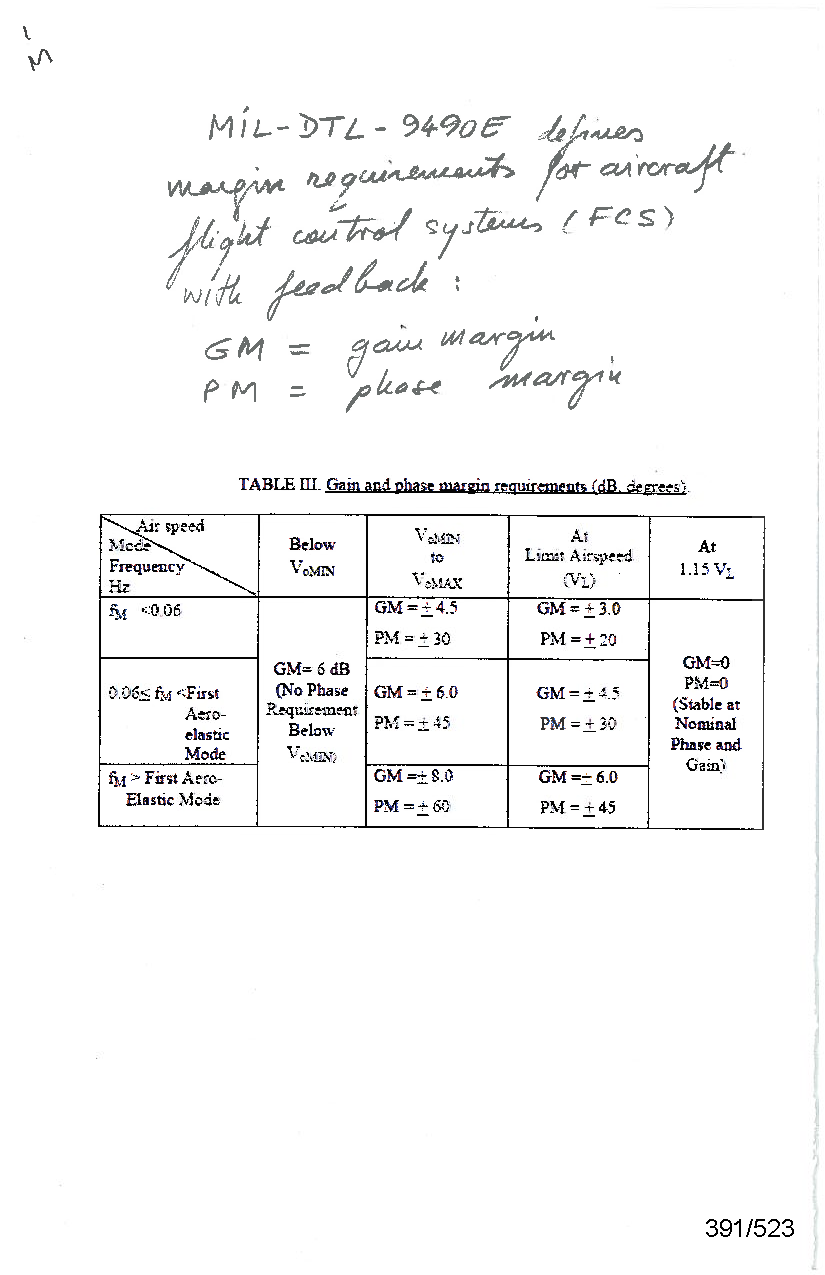
\includepdf[pages=-,pagecommand={},width=0.9\textwidth]{PDF_notes/Stability_Margins.pdf}

\subsection{Phase Compensators}
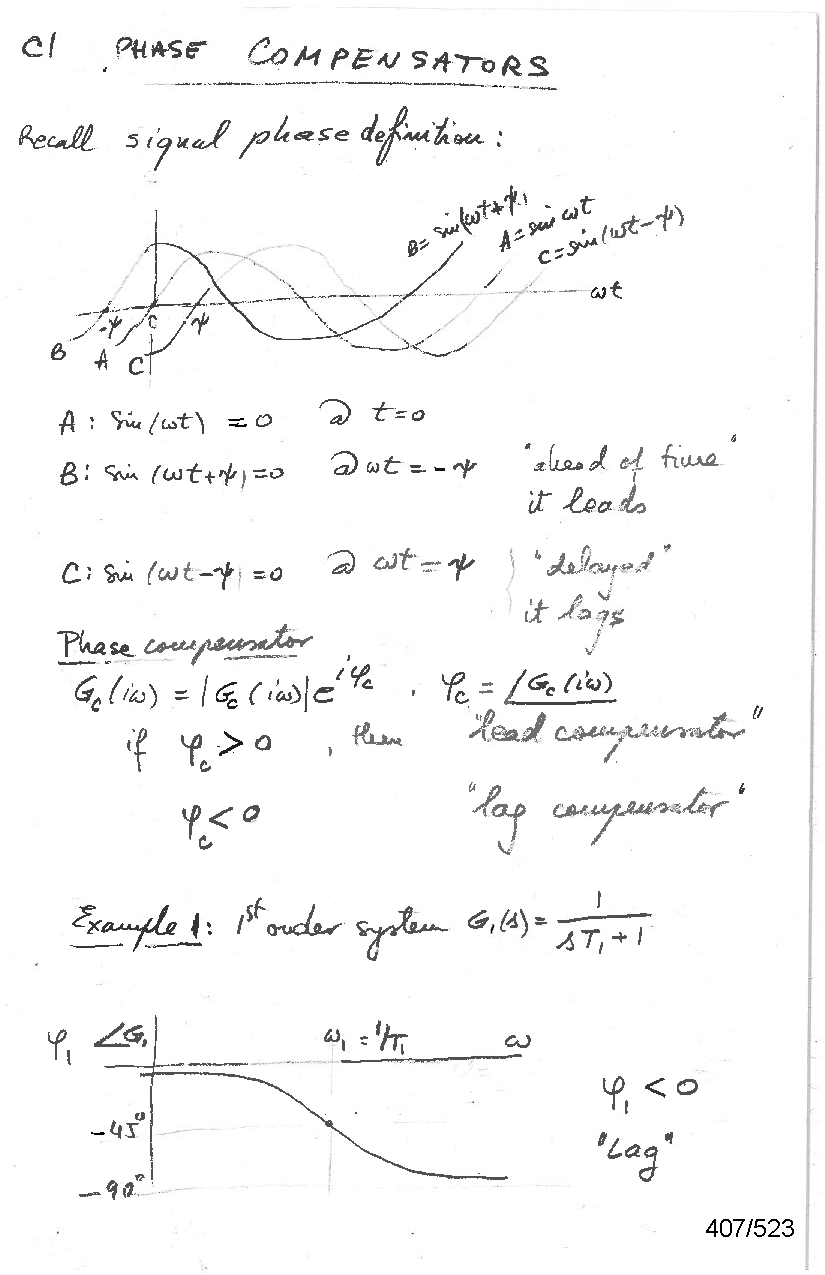
\includepdf[pages=-,pagecommand={},width=0.9\textwidth]{PDF_notes/Phase_Compensators.pdf}

\subsection{Lag Compensators}
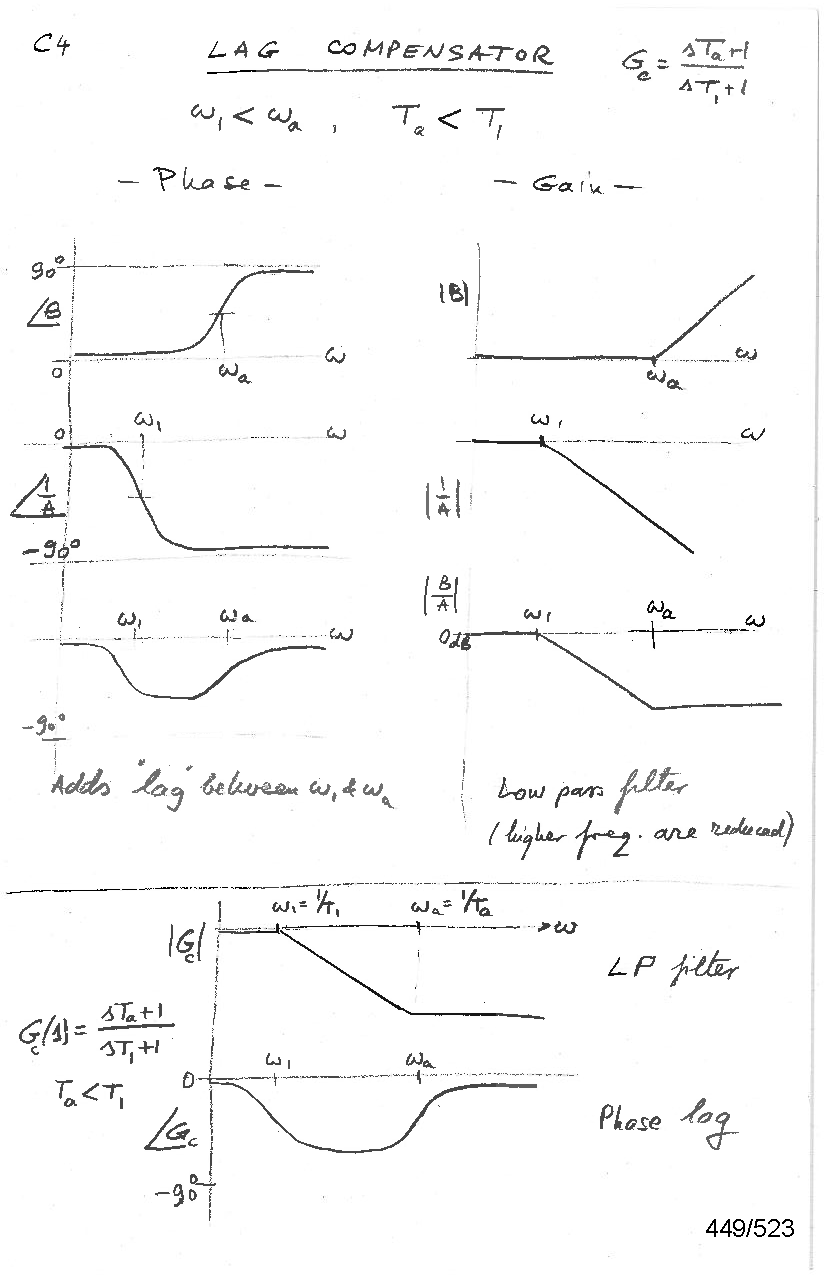
\includepdf[pages=-,pagecommand={},width=0.9\textwidth]{PDF_notes/Lag_Compensators.pdf}















	\pagebreak
	\renewcommand{\thepage}{}
	\renewcommand\refname{References Cited}
	\pagestyle{plain}
	\bibliographystyle{Downey_NSF}
	\bibliography{Chapter_1_Basic_Concepts}


















\end{document}

